\subsection{Investimento residencial nos modelos macroeconométricos}\label{RevEmpirica}

Compreendida a importância do investimento residencial para a dinâmica macroeconômica americana, faz-se necessária uma investigação dos determinantes deste gastos de acordo com a literatura econométrica e este é o objetivo desta seção. 
No entanto, dado o objeto desta pesquisa, destaca-se aqueles trabalhos que enfatizam a importância da construção de novos imóveis para o ciclo econômico para além da contribuição de \textcite{leamer_housing_2007}.


É importante pontuar que nos anos que procederam a crise do mercado imobiliário, verificou-se um crescente interesse nas implicações macroeconômicas do investimento residencial. Inspecionando modelos DSGE que incluem investimento residencial, \textcite{iacoviello_housing_2010} conclui que um melhor entendimento dos impactos deste gasto se faz necessária para a compreensão das flutuações macroeconômicas. Outros estudos, por sua vez, têm enfatizado o efeito riqueza sobre o consumo via valorização dos imóveis e indicam tais canais de transmissão são mais incidentes, em ordem, sobre Estados Unidos e Grã Bretanha mas mais brandos no caso francês e alemão \cites{sastre_assessment_2010}{chauvin_wealth_2010}{bassanetti_effects_2010}{arrondel_housing_2010}. 
\textcite{alvarez_does_2010}, por sua vez, concluem que tal tipo de investimento antecede o ciclo econômico para o caso de espanhol e resultados semelhantes podem ser encontrados para França, Espanha  e Itália enquanto na Alemanha esta dinâmica é distinta \cites{ferrara_common_2010}{ferrara_cyclical_2010}{ferrara_common_2010}\footnote{\textcite{alhowaish_causality_2015}, por outro lado, destaca que o investimento em infra-estrutura é induzido pelo setor petrolífero no caso da Arábia Saudita. Apesar de contrapor \textcite{green_follow_1997}  e \textcite{leamer_housing_2007}, tal resultado não é comparável uma vez que não é feita a devida distinção entre os gastos em construção civil feitos pelo governo e investimento residencial propriamente dito. Resultados semelhantes são obtidos por \textcite{ofori_testing_2003} em que investimento residencial também é somado ao investimento em infraestrutura.}. 

Um estudo que se sobressai é o de \textcite{arestis_residential_2015} em que é estendida a contribuição de \textcite{poterba_tax_1984} por meio de um modelo ARDL para 17 países da OCDE. Dentre as conclusões, destaca-se a importância da renda disponível como principal determinante do investimento residencial para os países em questão.  A implicação deste resultado, no entanto, questionaria a possibilidade de tratar o investimento residencial enquanto um gasto autônomo e, portanto, comprometeria a análise a partir do supermultiplicador sraffiano. Porém, tal resultado não é estatisticamente significante para o caso norte-americano em que o preço dos imóveis bem como o acesso ao crédito são os principais determinantes desse gasto e, desse modo, reaviva a discussão para a presente investigação.


Outro estudo recente é o de \textcite{huang_is_2018} em que os autores testam ambas as hipóteses aventadas por Leamer a despeito do investimento residencial (predição e causalidade). Para isso, estimam um modelo VAR estrutural (SVAR) com transformada \textit{wavelets} para os países da OCDE\footnote{
	Além de testar se a construção de novos imóveis antecipa movimentos no ciclo econômico, os autores também testam os canais de transmissão da política monetária em quatro frentes: (i) teoria neoclásica do investimento residencial; (ii) efeito riqueza do preço dos imóveis sobre o consumo por meio de um modelo de ciclo de vida; (iii) efeito do colateral sobre o balanço patrimonial das famílias e consumo; (iv) efeito do colateral sobre o balanço patrimonial dos bancos e oferta de crédito.}.  
Os autores concluem que o investimento residencial não é um mero canal de transmissão da política monetária e que possui efeitos temporalmente distintos sobre o ciclo econômico. No curto prazo, a construção de novos imóveis tem maior capacidade preditiva enquanto o preço dos imóveis tem maior influência no longo prazo\footnote{Adicionalmente, \textcite{huang_is_2018} também concluem que a capacidade preditiva do investimento residencial é maior quanto maior a parcela deste gasto no produto.}. A razão desta distinção, argumentam, é que a transmissão da política monetária via o canal da riqueza é mais proeminente no longo prazo enquanto os canais de crédito e de colateral são mais presentes no curto prazo. Já no que diz respeito a relação causal estabelecida por \textcite{leamer_housing_2007}, afirmam que os resultados não são conclusivos para todos os países diante da heterogeneidade institucional observada\footnote{
	No entanto, os autores afirmam que para a maioria dos países do G7 o investimento residencial é ao menos capaz de amplificar o ciclo econômico.}, mas ainda é valida para os Estados Unidos\footnote{
	Apenas para ilustrar a dimensão da importância do investimento residencial para o ciclo econômio norte-americano, \textcite{huang_is_2018} utilizam este pais como critério de comparação.}.
Apesar dos resultados não conclusivos sobre as flutuações, concluem que as variáveis associadas ao investimento residencial (preço dos imóveis, taxa real de juros das hipotecas --- deflacionada pelo índice de preços --- e \textit{spread} bancário) lideram o crescimento econômico.

%Retomada Green e Leamer
Apesar de significativos, os resultados  de \textcite{huang_is_2018} reportados acima incorrem em uma imprecisão a despeito da taxa de juros selecionada para avaliar os impactos sobre o investimento residencial. 
MAIS CRÍTICAS AO HUANG ET AL.


ESTES ESTUDOS INDICAM A RELEVÂNCIA DO INVESTIMENTO RESIDENCIAL PARA A DINÂMICA.

Jean Gauger \& Tricia Coxwell Snyder

COMENTÁRIO SOBRE A TAXA PRÓPRIA

Para evidenciar esta relação, o gráfico \ref{gZ_Propria} ilustra como  o deflacionamento da taxa de juros hipotecária pelo preço dos imóveis --- e não por um índice de preços generalizado como em \textcite[p.~143--146]{fair_macroeconometric_2013} --- é mais adequado para captar a dinâmica do investimento residencial. Tal proposição, no entanto, não é avaliada por meio da estimação de um modelo empírico. Desse modo, a seção seguinte pretende verificar a capacidade explicativa desta alternativa.

%TODO Alterar imagem


\begin{figure}[H]
	\centering
	\caption{Taxa real e própria de juros dos imóveis x investimento residencial}
	\label{gZ_Propria}
	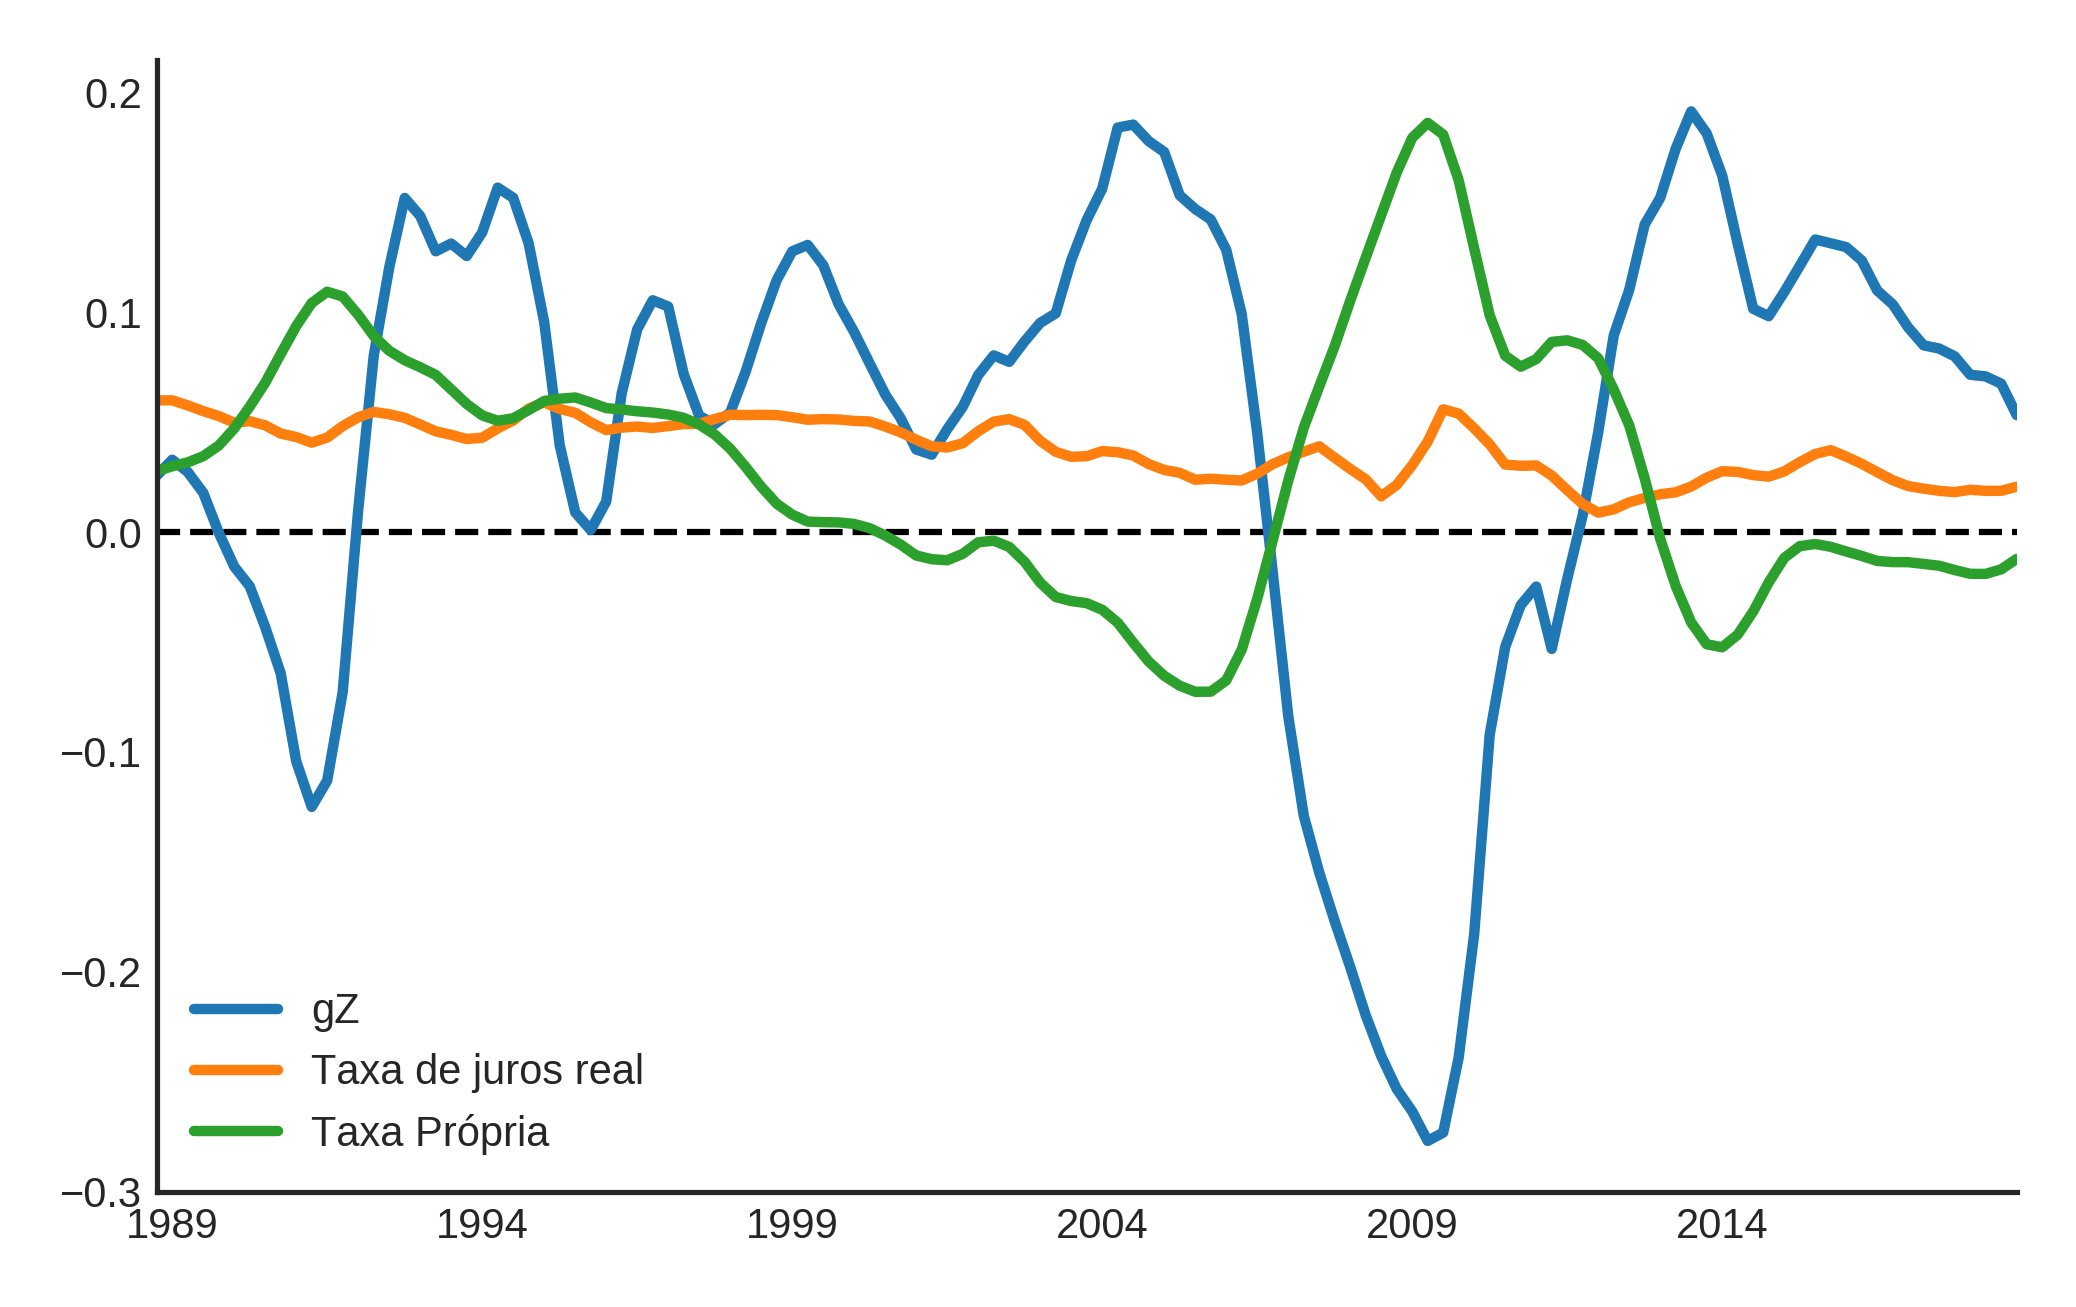
\includegraphics[width=0.75\textwidth]{Fatos_Estilizados/Figs/TxPropria_Investo.png}
	\caption*{\textbf{Fonte:} U.S. Bureau of Economic Analysis, elaboração própria}
\end{figure}
